\section{Introduction}

\begin{figure}
    \centering
    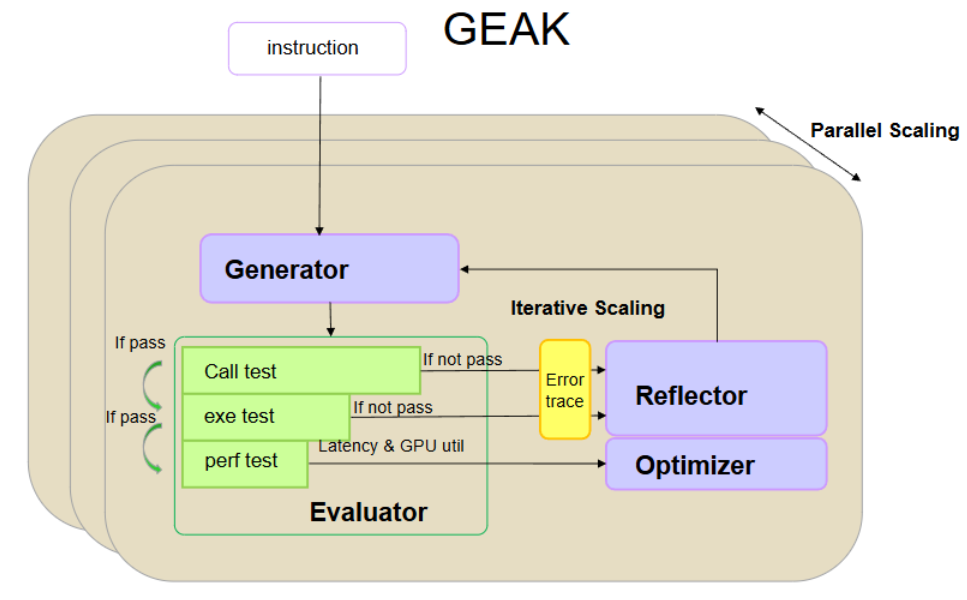
\includegraphics[width=0.95\linewidth]{figures/GEAK_pipeline.png}
    \caption{Illustration of GEAK pipeline.}
    \label{fig:geak-pipeline}
\end{figure}

As AI workloads scale in both complexity and hardware diversity, there is a growing demand for intelligent systems that can generate high-performance GPU kernels without manual tuning. This demand is especially critical in environments where tight coupling between software and hardware efficiency determines practical feasibility—ranging from hyperscaler data centers used for serving frontier LLMs to academic HPC clusters. Recent advances in large language models (LLMs) have shown promising capabilities in code generation tasks, but achieving correct and efficient GPU code remains an open challenge. AI-assisted GPU kernel development, particularly for emerging hardware like AMD Instinct™ MI300X GPUs, can substantially improve productivity and deployment speed.

To this end, we introduce GEAK (Generating Efficient AI-centric GPU Kernels), AMD’s new agentic framework for automatic Triton kernel generation targeting AMD Instinct™ GPUs. GEAK is built to push the frontier of AI-assisted code generation by combining state-of-the-art LLMs with a structured reasoning and feedback loop. Alongside GEAK, we release two benchmark suites for evaluating AI-generated Triton kernels, enabling measurement of both execution correctness and runtime performance of generated kernels.

\textbf{Key Contributions:}
\begin{enumerate}
    \item We introduce \textbf{GEAK framework}, a modular, agent-based system that uses inference-time compute scaling with frontier LLMs to generate Triton GPU kernels from minimal task descriptions. GEAK incorporates multiple agents—generation, evaluation, reflection, and optimization—to iteratively refine code quality and execution performance.
    \item We establish two benchmark suites for evaluating Triton kernel generation. The \textbf{TritonBench-revised} is a revised subset of 184 kernels adapted from TritonBench-G\cite{li2025tritonbenchbenchmarkinglargelanguage} with stricter testing harnesses. In addition, we release the \textbf{ROCm Triton Benchmark}, a new suite of 30 real-world kernels sampled from open-source AMD ROCm repositories.
    \item We demonstrate that GEAK significantly outperforms direct prompting of state-of-the-art LLMs, achieving correct kernel generation rate up to $54.89$\% on TritonBench-revised and $63.33$\% on the ROCm Triton benchmark—compared to less than $15$\% when directly prompting strong LLMs without agentic feedback.
    \item We also present a detailed study on one of the performant kernels from ROCm Triton Benchmark (please see Appendix \ref{appendix:case-study}).
    \item We open source our GEAK agent implementation (\href{https://github.com/AMD-AIG-AIMA/GEAK-agent}{github link}) and GEAK evaluation framework (\href{https://github.com/AMD-AIG-AIMA/GEAK-eval}{github link}).
\end{enumerate}

Furthermore, GEAK-generated kernels demonstrate an average speedup of up to $2.59$× over their reference counterparts on the TritonBench-revised set. 